% Created 2019-05-22 Wed 11:16
% Intended LaTeX compiler: pdflatex
\documentclass[a4paper]{article}
\usepackage[utf8]{inputenc}
\usepackage[T1]{fontenc}
\usepackage{graphicx}
\usepackage{grffile}
\usepackage{longtable}
\usepackage{wrapfig}
\usepackage{rotating}
\usepackage[normalem]{ulem}
\usepackage{amsmath}
\usepackage{textcomp}
\usepackage{amssymb}
\usepackage{capt-of}
\usepackage{hyperref}
\usepackage{minted}
\usepackage[margin=0.8in]{geometry}
\usepackage{amssymb,amsmath}
\usepackage{fancyhdr}
\pagestyle{fancy}
\usepackage{lastpage}
\usepackage{float}
\restylefloat{figure}
\usepackage{hyperref}
\usepackage{tabularx}
\hypersetup{urlcolor=blue}
\usepackage{titlesec}
\setcounter{secnumdepth}{4}
\usepackage{minted}
\setminted{frame=single,framesep=10pt}
\chead{}
\rhead{\today}
\cfoot{}
\rfoot{\thepage\ of \pageref{LastPage}}
\usepackage[parfill]{parskip}
\usepackage{subfig}
\usepackage[sort&compress, numbers]{natbib}
\hypersetup{colorlinks=true,linkcolor=black, citecolor=black}
\usepackage{framed}
\usepackage{mathtools, cases}
\author{Nathan Hughes (JIC)}
\date{\today}
\title{RNA-seq Report}
\hypersetup{
 pdfauthor={Nathan Hughes (JIC)},
 pdftitle={RNA-seq Report},
 pdfkeywords={},
 pdfsubject={},
 pdfcreator={Emacs 26.1 (Org mode 9.1.9)},
 pdflang={English}}
\begin{document}

\maketitle
\maketitle
\clearpage
\tableofcontents
\clearpage



\section{Intro + example data}
\label{sec:orga9cbabb}


\subsection{Examples of data}
\label{sec:orgfc96b3e}

\subsubsection{Normalised count data}
\label{sec:orgffc340f}

\begin{center}
\begin{tabular}{lrrrr}
 & cer\_c\_05h\_a37 & cer\_c\_05h\_b38 & cer\_c\_05h\_c39 & cer\_c\_6h\_a85\\
\hline
AT1G57560 & 6.66594 & 6.86016 & 6.71742 & 7.03654\\
AT2G03260 & 6.97298 & 7.08292 & 6.73242 & 6.89541\\
AT2G36355 & 7.53624 & 7.24664 & 7.22017 & 7.3226\\
AT1G11185 & 7.44287 & 7.37075 & 7.32766 & 6.51549\\
AT5G23030 & 6.06316 & 6.35515 & 6.21125 & 6.12698\\
AT5G16520 & 7.66076 & 7.63511 & 7.5679 & 7.40679\\
AT4G33150 & 9.03895 & 9.07082 & 9.05513 & 9.35499\\
AT4G14630 & 8.05476 & 8.24193 & 8.07485 & 7.42149\\
AT3G14560 & 7.08607 & 7.13215 & 7.1723 & 7.31465\\
AT1G18590 & 9.10513 & 8.96686 & 9.02159 & 9.35499\\
AT5G05365 & 8.09272 & 8.31546 & 7.93893 & 7.69591\\
AT5G11160 & 7.54439 & 7.81302 & 7.70158 & 7.61088\\
AT1G27420 & 7.12133 & 6.72751 & 6.53351 & 7.29047\\
AT5G18270 & 7.9986 & 7.83365 & 7.70791 & 7.24903\\
AT1G80440 & 6.8464 & 6.93494 & 6.83126 & 7.4786\\
AT1G07970 & 7.98129 & 8.0474 & 8.10328 & 8.20224\\
AT1G55450 & 10.1205 & 10.3351 & 10.2424 & 9.58924\\
AT5G24840 & 8.21536 & 8.27673 & 8.22432 & 8.19418\\
AT2G37460 & 8.14517 & 8.3438 & 8.19834 & 7.99419\\
AT2G07595 & 6.10621 & 6.02556 & 5.99113 & 5.97591\\
\end{tabular}
\end{center}

\subsubsection{Expression difference hypothesis tests}
\label{sec:orge10bfd4}

\begin{center}
\begin{tabular}{lrrrrrrl}
gene & baseMean & log2FoldChange & lfcSE & stat & pvalue & padj & sample\\
\hline
AT5G39090 & 13.2487 & 0.9219 & 0.594288 & 1.55127 & 0.120838 & 0.335167 & cer\_w\_05h\\
AT5G14380 & 8.87757 & -1.17008 & 0.659602 & -1.77391 & 0.0760777 & 0.257841 & cer\_w\_6h\\
AT1G19730 & 119.519 & -0.021061 & 0.203546 & -0.10347 & 0.91759 & 0.968718 & col\_c\_05h\\
AT1G05493 & 4.37256 & 0.191672 & 0.96016 & 0.199625 & 0.841774 & 0.933395 & lym\_c\_05h\\
AT3G09032 & 22.053 & 0.399712 & 0.48984 & 0.816006 & 0.414497 & 0.676983 & cer\_c\_05h\\
AT2G41375 & 45.7757 & 0.0301228 & 0.31699 & 0.0950276 & 0.924293 & 0.971808 & cer\_c\_6h\\
AT4G36180 & 257.118 & 0.121669 & 0.189834 & 0.640924 & 0.521572 & 0.863141 & col\_w\_6h\\
AT1G23210 & 5.9605 & 0.155948 & 0.988455 & 0.157769 & 0.874639 & 0.951012 & col\_c\_05h\\
AT2G01750 & 254.113 & -0.313262 & 0.140221 & -2.23405 & 0.0254795 & 0.119981 & col\_c\_05h\\
AT2G18780 & 17.807 & 0.149322 & 0.570296 & 0.261832 & 0.793451 & 0.905366 & col\_c\_6h\\
AT1G17410 & 46.0602 & -0.101394 & 0.267701 & -0.378756 & 0.704869 & 0.858978 & col\_c\_6h\\
AT4G39330 & 1441.72 & -0.0939816 & 0.0989497 & -0.949792 & 0.342218 & 0.863757 & lym\_w\_05h\\
AT4G38130 & 1203.39 & 0.00369207 & 0.0794837 & 0.0464507 & 0.962951 & 0.998246 & lym\_w\_05h\\
AT3G52190 & 273.452 & 0.55585 & 0.161152 & 3.44924 & 0.000562174 & 0.00753138 & cer\_w\_6h\\
AT3G12270 & 323.137 & 0.377735 & 0.153265 & 2.46459 & 0.0137171 & 0.0821683 & cer\_w\_05h\\
AT4G24805 & 199.389 & 0.6758 & 0.150516 & 4.4899 & 7.12563\,(-06) & 7.87341\,(-05) & lym\_c\_05h\\
AT3G05430 & 32.4406 & 0.350837 & 0.362139 & 0.96879 & 0.33265 & 0.859876 & lym\_w\_05h\\
AT3G01135 & 43.5689 & -0.379412 & 0.268763 & -1.4117 & 0.158039 & 0.421368 & cer\_c\_6h\\
AT3G13404 & 6.12748 & -0.193849 & 0.861789 & -0.224938 & 0.822028 & 0.925835 & cer\_w\_6h\\
AT2G24860 & 270.011 & -0.174685 & 0.160757 & -1.08664 & 0.277195 & 0.715961 & col\_w\_6h\\
\end{tabular}
\end{center}

\subsubsection{Data with extra descriptions}
\label{sec:org894a806}
\begin{center}
\begin{tabular}{rllrrllll}
 & incoming & converted & n\_incoming & n\_converted & name & description & namespaces & query\\
\hline
0 & AT2G47410 & AT2G47410 & 1 & 1 & AT2G47410 & WD40/YVTN repeat-like-containing domain & ARRAYEXPRESS,ENSG,NASC\_GENE\_ID\_ACC,TAIR\_LOCUS,TAIR\_TRANSLATION & query\_1\\
1 & AT1G16730 & AT1G16730 & 2 & 1 & UP6 & F17F16.6 protein & ARRAYEXPRESS,ENSG,NASC\_GENE\_ID\_ACC,TAIR\_LOCUS,TAIR\_TRANSLATION & query\_1\\
2 & AT2G17850 & AT2G17850 & 3 & 1 & AT2G17850 & Rhodanese/Cell cycle control phosphatase superfamily protein & ARRAYEXPRESS,ENSG,NASC\_GENE\_ID\_ACC,TAIR\_LOCUS,TAIR\_TRANSLATION & query\_1\\
3 & AT3G59410 & AT3G59410 & 4 & 1 & GCN2 & Protein kinase family protein & ARRAYEXPRESS,ENSG,NASC\_GENE\_ID\_ACC,TAIR\_LOCUS,TAIR\_TRANSLATION & query\_1\\
4 & AT1G02930 & AT1G02930 & 5 & 1 & GSTF6 & Glutathione S-transferase F6 & ARRAYEXPRESS,ENSG,NASC\_GENE\_ID\_ACC,TAIR\_LOCUS,TAIR\_TRANSLATION & query\_1\\
5 & AT3G09970 & AT3G09970 & 6 & 1 & AT3G09970 & Calcineurin-like metallo-phosphoesterase superfamily protein & ARRAYEXPRESS,ENSG,NASC\_GENE\_ID\_ACC,TAIR\_LOCUS,TAIR\_TRANSLATION & query\_1\\
6 & AT2G13840 & AT2G13840 & 7 & 1 & AT2G13840 & Expressed protein & ARRAYEXPRESS,ENSG,NASC\_GENE\_ID\_ACC,TAIR\_LOCUS,TAIR\_TRANSLATION & query\_1\\
7 & AT4G00355 & AT4G00355 & 8 & 1 & ATI2 & ATG8-interacting protein 2 & ARRAYEXPRESS,ENSG,NASC\_GENE\_ID\_ACC,TAIR\_LOCUS,TAIR\_TRANSLATION & query\_1\\
8 & AT4G26380 & AT4G26380 & 9 & 1 & AT4G26380 & Cysteine/Histidine-rich C1 domain family protein & ARRAYEXPRESS,ENSG,NASC\_GENE\_ID\_ACC,TAIR\_LOCUS,TAIR\_TRANSLATION & query\_1\\
9 & AT5G01435 & AT5G01435 & 10 & 1 & AT5G01435 & None & ARRAYEXPRESS,ENSG & query\_1\\
10 & AT4G38825 & AT4G38825 & 11 & 1 & AT4G38825 & SAUR-like auxin-responsive protein family & ARRAYEXPRESS,ENSG,NASC\_GENE\_ID\_ACC,TAIR\_LOCUS,TAIR\_TRANSLATION & query\_1\\
11 & AT3G54220 & AT3G54220 & 12 & 1 & SCR & Protein SCARECROW & ARRAYEXPRESS,ENSG,NASC\_GENE\_ID\_ACC,TAIR\_LOCUS,TAIR\_TRANSLATION & query\_1\\
12 & AT2G44020 & AT2G44020 & 13 & 1 & AT2G44020 & Expressed protein & ARRAYEXPRESS,ENSG,NASC\_GENE\_ID\_ACC,TAIR\_LOCUS,TAIR\_TRANSLATION & query\_1\\
13 & AT5G15170 & AT5G15170 & 14 & 1 & TDP1 & Tyrosyl-DNA phosphodiesterase 1 & ARRAYEXPRESS,ENSG,NASC\_GENE\_ID\_ACC,TAIR\_LOCUS,TAIR\_TRANSLATION & query\_1\\
14 & AT2G36360 & AT2G36360 & 15 & 1 & AT2G36360 & Galactose oxidase/kelch repeat superfamily protein & ARRAYEXPRESS,ENSG,NASC\_GENE\_ID\_ACC,TAIR\_LOCUS,TAIR\_TRANSLATION & query\_1\\
15 & AT1G78780 & AT1G78780 & 16 & 1 & AT1G78780 & pathogenesis-related family protein & ARRAYEXPRESS,ENSG,NASC\_GENE\_ID\_ACC,TAIR\_LOCUS,TAIR\_TRANSLATION & query\_1\\
16 & AT4G23460 & AT4G23460 & 17 & 1 & BETAC-AD & Beta-adaptin-like protein C & ARRAYEXPRESS,ENSG,NASC\_GENE\_ID\_ACC,TAIR\_LOCUS,TAIR\_TRANSLATION & query\_1\\
17 & AT4G00300 & AT4G00300 & 18 & 1 & AT4G00300 & Receptor-like kinase & ARRAYEXPRESS,ENSG,NASC\_GENE\_ID\_ACC,TAIR\_LOCUS,TAIR\_TRANSLATION & query\_1\\
18 & AT1G71130 & AT1G71130 & 19 & 1 & ERF070 & Ethylene-responsive transcription factor ERF070 & ARRAYEXPRESS,ENSG,NASC\_GENE\_ID\_ACC,TAIR\_LOCUS,TAIR\_TRANSLATION & query\_1\\
19 & AT3G04000 & AT3G04000 & 20 & 1 & ChlADR2 & NADPH-dependent aldehyde reductase 2, chloroplastic & ARRAYEXPRESS,ENSG,NASC\_GENE\_ID\_ACC,TAIR\_LOCUS,TAIR\_TRANSLATION & query\_1\\
\end{tabular}
\end{center}

\clearpage
\section{Initial data checking}
\label{sec:org490c813}

\subsection{Check sample counts}
\label{sec:org4e1d870}
This shows that the normalisation of the count data has worked correctly, each sample is presented as having the same number of reads.
This prevents different samples having different weights due to RNA-seq not producing uniform samples.

\begin{verbatim}
<Figure size 720x720 with 1 Axes>
\end{verbatim}

\begin{figure}[htbp]
\centering
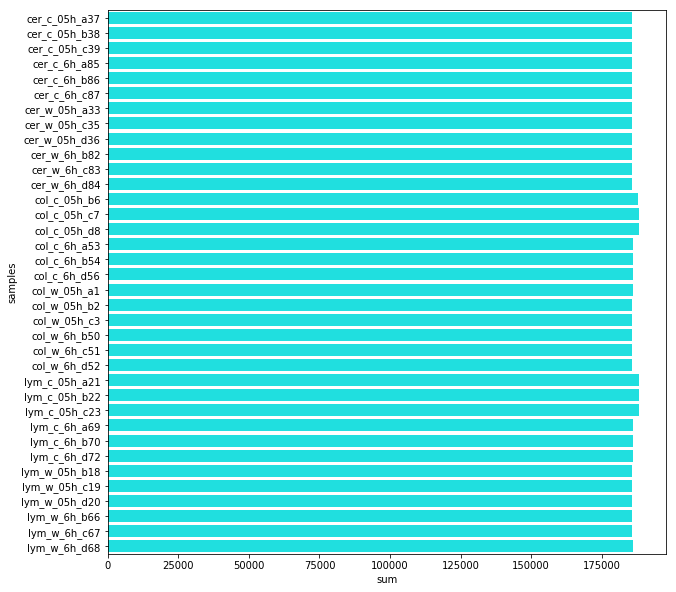
\includegraphics[width=.9\linewidth]{obipy-resources/samplecounts.png}
\caption{\label{samplecounts}
Counting the number of reads found in each sample}
\end{figure}

\clearpage


\subsection{Check for sample differences}
\label{sec:org0f25176}
Here, we do a naive check that there is variance within the samples; this matrix shows that a straight-forward euclidean distance of all counts in the samples are different. i.e. if there was a very small difference here it would be worrying and suggest that there isn't any significant changes.
This figure is a simple data sanity check, \textbf{not of use for scientific purposes}.

NameErrorTraceback (most recent call last)
<ipython-input-11-16720fa86bb7> in <module>
     17 \#legend\_TN = [mpatches.Patch(color=c, label=l) for (list(set([c[:3] for c in collapsed\_counts.columns]))]
     18
---> 19 distances = pdist(collapsed\_counts.T.values, metric='euclidean')
     20 dist\_matrix = squareform(distances)
     21 dist\_df = pd.DataFrame(dist\_matrix, columns = collapsed\_counts.columns, index=collapsed\_counts.columns)

NameError: name 'pdist' is not defined

\clearpage
\section{Analysis}
\label{sec:org38f601f}

\subsection{Comparing 05hr chitin to water treatments}
\label{sec:org0933277}

\subsubsection{Clustermap of largest/smallest DE genes}
\label{sec:org1618a07}
\begin{verbatim}
<Figure size 720x720 with 4 Axes>
\end{verbatim}

\begin{center}
\includegraphics[width=.9\linewidth]{obipy-resources/9cd72325f5feb94da5a4a2bf9cf66bfba3128720/64b51c1cbc1e5d4112f6b391f5f33b91f8774633.png}
\end{center}

\begin{verbatim}
<Figure size 720x720 with 4 Axes>
\end{verbatim}

\begin{center}
\includegraphics[width=.9\linewidth]{obipy-resources/9cd72325f5feb94da5a4a2bf9cf66bfba3128720/f1d5bf9ebf5510461deba3e9ea7334988f295e15.png}
\end{center}



\subsubsection{Boxplots of differential changes}
\label{sec:orgeedf0bb}

\begin{verbatim}
<Figure size 1080x360 with 2 Axes>
\end{verbatim}

\begin{figure}[htbp]
\centering
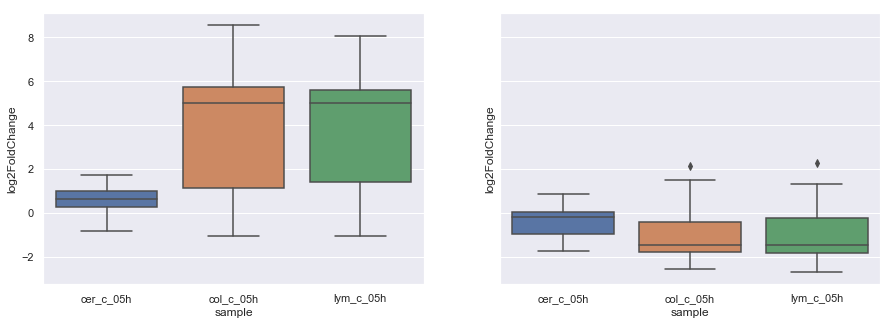
\includegraphics[width=.9\linewidth]{obipy-resources/pairings_05hr_boxplots.png}
\caption{\label{pairings_05hr_boxplots}
Boxplots of differential expressions from 50 largest (left) and 50 lowe05hst (right) DE genes}
\end{figure}


\clearpage

\subsection{Comparing 6hr chitin to water treatments}
\label{sec:org6ab7a03}

\subsubsection{Clustermap of largest/smallest DE genes}
\label{sec:org349ce79}
\begin{verbatim}
<Figure size 720x720 with 4 Axes>
\end{verbatim}

\begin{center}
\includegraphics[width=.9\linewidth]{obipy-resources/9cd72325f5feb94da5a4a2bf9cf66bfba3128720/a7bd280b6a85e3544fc81c603a6243f9f82eb888.png}
\end{center}

\begin{verbatim}
<Figure size 720x720 with 4 Axes>
\end{verbatim}

\begin{center}
\includegraphics[width=.9\linewidth]{obipy-resources/9cd72325f5feb94da5a4a2bf9cf66bfba3128720/08c8c5f37494d9b646ffd479ad1db0ac175106aa.png}
\end{center}

\subsubsection{Boxplots of differential changes}
\label{sec:org20253f0}

\begin{verbatim}
<Figure size 1080x360 with 2 Axes>
\end{verbatim}

\begin{figure}[htbp]
\centering
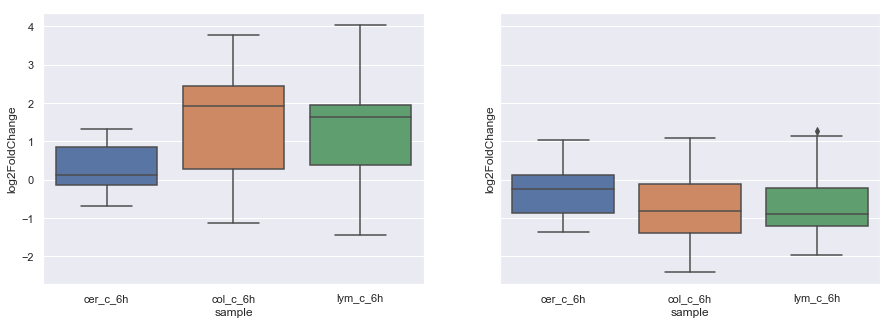
\includegraphics[width=.9\linewidth]{obipy-resources/pairings_6hr_boxplots.png}
\caption{\label{pairings_6hr_boxplots}
Boxplots of differential expressions from 50 largest (left) and 50 lowest (right) DE genes}
\end{figure}



\clearpage
\subsection{Comparing 05hr treatments to lym}
\label{sec:org7d44aa0}

\subsubsection{Clustermap of largest/smallest DE genes}
\label{sec:org6109b0f}
\begin{verbatim}
<Figure size 720x720 with 4 Axes>
\end{verbatim}

\begin{center}
\includegraphics[width=.9\linewidth]{obipy-resources/9cd72325f5feb94da5a4a2bf9cf66bfba3128720/59db26fd12b341fe438b64d3f155a63a90695e85.png}
\end{center}

\begin{verbatim}
<Figure size 720x720 with 4 Axes>
\end{verbatim}

\begin{center}
\includegraphics[width=.9\linewidth]{obipy-resources/9cd72325f5feb94da5a4a2bf9cf66bfba3128720/8276239e9ae27707edfee10548406edf576eac5e.png}
\end{center}

\subsubsection{Boxplots of differential changes}
\label{sec:org1965ec5}

\begin{verbatim}
<Figure size 1080x360 with 2 Axes>
\end{verbatim}

\begin{figure}[htbp]
\centering
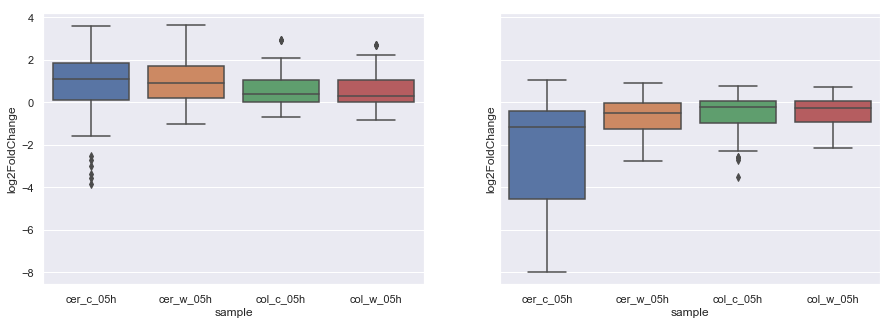
\includegraphics[width=.9\linewidth]{obipy-resources/pairings_05hr_lym_boxplots.png}
\caption{\label{pairings_05hr_lym_boxplots}
Boxplots of differential expressions from 50 largest (left) and 50 lowest (right) DE genes}
\end{figure}


\clearpage
\subsection{Comparing 6hr treatments to lym}
\label{sec:org2607aa3}
\subsubsection{Clustermap of largest/smallest DE genes}
\label{sec:org4eb618e}
\begin{verbatim}
<Figure size 720x720 with 4 Axes>
\end{verbatim}

\begin{center}
\includegraphics[width=.9\linewidth]{obipy-resources/9cd72325f5feb94da5a4a2bf9cf66bfba3128720/a828d5e435d435dc3cb8524d5cdb1871265369fd.png}
\end{center}

\begin{verbatim}
<Figure size 720x720 with 4 Axes>
\end{verbatim}

\begin{center}
\includegraphics[width=.9\linewidth]{obipy-resources/9cd72325f5feb94da5a4a2bf9cf66bfba3128720/f6b62fef4158e761352c1841a1a9ff9d7946e0e3.png}
\end{center}


\subsubsection{Boxplots of differential changes}
\label{sec:orgafd91a7}

\begin{verbatim}
<Figure size 1080x360 with 2 Axes>
\end{verbatim}

\begin{figure}[htbp]
\centering
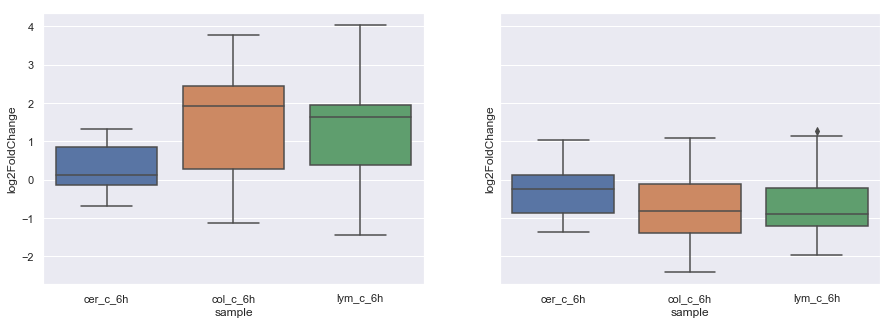
\includegraphics[width=.9\linewidth]{obipy-resources/pairings_6hr_lym_boxplots.png}
\caption{\label{pairings_6hr_lym_boxplots}
Boxplots of differential expressions from 50 largest (left) and 50 lowest (right) DE genes}
\end{figure}


\clearpage
\subsection{Comparing all treatments across time}
\label{sec:orgedc71f0}
\subsubsection{Clustermap of largest/smallest DE genes}
\label{sec:org817d5b8}
\begin{verbatim}
<Figure size 720x720 with 4 Axes>
\end{verbatim}

\begin{center}
\includegraphics[width=.9\linewidth]{obipy-resources/9cd72325f5feb94da5a4a2bf9cf66bfba3128720/75adc85bc64db8458b069cf3d3fc9882f28e1d78.png}
\end{center}

\begin{verbatim}
<Figure size 720x720 with 4 Axes>
\end{verbatim}

\begin{center}
\includegraphics[width=.9\linewidth]{obipy-resources/9cd72325f5feb94da5a4a2bf9cf66bfba3128720/b3bcc20aa5ee2c7db70b61562e18a41bbd8a2293.png}
\end{center}


\subsubsection{Boxplots of differential changes}
\label{sec:org874876e}

\begin{verbatim}
<Figure size 1080x360 with 2 Axes>
\end{verbatim}

\begin{figure}[htbp]
\centering
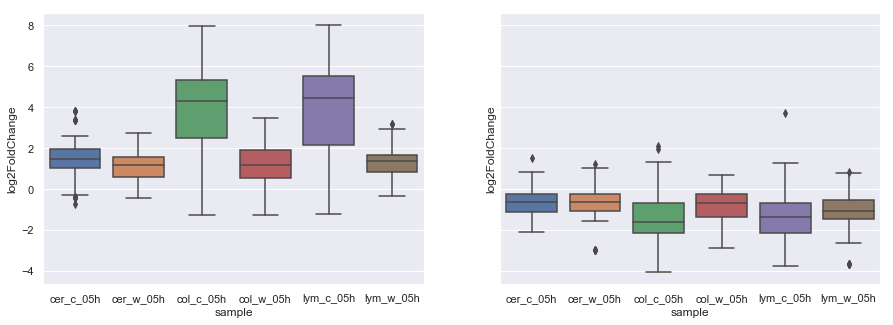
\includegraphics[width=.9\linewidth]{obipy-resources/pairings_timingsr_boxplots.png}
\caption{\label{pairings_timings_boxplots}
Boxplots of differential expressions from 50 largest (left) and 50 lowest (right) DE genes}
\end{figure}

\subsubsection{Lineplots of changes between samples for genes of interest}
\label{sec:org0c7b177}
\begin{verbatim}
<Figure size 1440x720 with 10 Axes>
\end{verbatim}

\begin{center}
\includegraphics[width=.9\linewidth]{obipy-resources/9cd72325f5feb94da5a4a2bf9cf66bfba3128720/6eaa3cec89bd95c2d331c8225791ae85dc358a4d.png}
\end{center}

\begin{verbatim}
<Figure size 1440x720 with 10 Axes>
\end{verbatim}

\begin{center}
\includegraphics[width=.9\linewidth]{obipy-resources/9cd72325f5feb94da5a4a2bf9cf66bfba3128720/d8eb75aab6d13c1d005f917f5d4167d0624708d9.png}
\end{center}

\begin{verbatim}
<Figure size 1440x720 with 10 Axes>
\end{verbatim}

\begin{center}
\includegraphics[width=.9\linewidth]{obipy-resources/9cd72325f5feb94da5a4a2bf9cf66bfba3128720/e14b2a50c52c0c53091783c9b195bc9f8f652ad3.png}
\end{center}

\begin{verbatim}
<Figure size 1440x720 with 10 Axes>
\end{verbatim}

\begin{center}
\includegraphics[width=.9\linewidth]{obipy-resources/9cd72325f5feb94da5a4a2bf9cf66bfba3128720/3a9ebe21758d975b29d5e81f6a4505b9b6a2d5b7.png}
\end{center}

\begin{verbatim}
<Figure size 1440x720 with 10 Axes>
\end{verbatim}

\begin{center}
\includegraphics[width=.9\linewidth]{obipy-resources/9cd72325f5feb94da5a4a2bf9cf66bfba3128720/9e0357b87776e45d8f87168fe006bce0f2131213.png}
\end{center}

\begin{verbatim}
<Figure size 1440x720 with 10 Axes>
\end{verbatim}

\begin{center}
\includegraphics[width=.9\linewidth]{obipy-resources/9cd72325f5feb94da5a4a2bf9cf66bfba3128720/b9adbbd55a75970a69346e600582d8b4d37d37dc.png}
\end{center}


\subsubsection{Checking up and down data's largest}
\label{sec:org5d34bc6}

\begin{center}
\begin{tabular}{llrrrrrrrrrrrr}
 & sample & baseMean & log2FoldChange & lfcSE & stat & pvalue & padj & lym\_c\_05h\_a21 & lym\_c\_05h\_b22 & lym\_c\_05h\_c23 & lym\_c\_6h\_a69 & lym\_c\_6h\_b70 & lym\_c\_6h\_d72\\
\hline
AT4G31950 & lym\_c\_05h & 62.134 & 11.1474 & 1.19661 & 9.31583 & 1.21003\,(-20) & 3.04446\,(-19) & 9.02695 & 8.85273 & 8.77664 & 5.60783 & 5.60783 & 5.60783\\
AT4G18540 & lym\_c\_05h & 49.8177 & 11.0383 & 2.57567 & 4.28561 & 1.82236\,(-05) & 0.000143129 & 8.77444 & 8.64281 & 8.96563 & 5.60783 & 5.60783 & 5.60783\\
AT1G05767 & lym\_c\_05h & 39.595 & 10.5272 & 1.20735 & 8.7192 & 2.80169\,(-18) & 6.36071\,(-17) & 8.51408 & 8.23432 & 8.45238 & 5.60783 & 5.60783 & 5.60783\\
AT1G47130 & lym\_c\_05h & 24.3826 & 9.55227 & 1.23862 & 7.71201 & 1.23856\,(-14) & 2.32962\,(-13) & 7.73677 & 7.55839 & 7.8844 & 5.60783 & 5.60783 & 5.60783\\
AT3G02840 & lym\_c\_05h & 498.838 & 9.44554 & 0.726166 & 13.0074 & 1.11048\,(-38) & 4.82548\,(-37) & 11.4503 & 11.3644 & 11.5624 & 5.60783 & 5.86799 & 6.28538\\
AT4G31970 & lym\_c\_05h & 107.475 & -8.72719 & 1.60424 & -5.44009 & 5.32543\,(-08) & 6.00415\,(-07) & 5.84268 & 5.60783 & 5.83302 & 9.51599 & 8.13272 & 7.91314\\
AT1G31173 & lym\_c\_05h & 29.224 & -7.94445 & 1.221 & -6.50649 & 7.69248\,(-11) & 1.12916\,(-09) & 5.60783 & 5.60783 & 5.60783 & 7.04642 & 6.68769 & 7.24795\\
AT3G60140 & lym\_c\_05h & 34.3907 & -6.2782 & 1.08995 & -5.76011 & 8.40611\,(-09) & 1.03509\,(-07) & 5.93959 & 5.94093 & 5.60783 & 7.63482 & 7.20347 & 8.33776\\
AT4G38850 & lym\_c\_05h & 6.02148 & -5.34424 & 1.36622 & -3.91169 & 9.16526\,(-05) & 0.000633583 & 5.60783 & 5.60783 & 5.60783 & 6.27229 & 6.24086 & 6.0387\\
AT5G03310 & lym\_c\_05h & 2.43405 & -5.16479 & 1.7501 & -2.95114 & 0.00316608 & 0.0146648 & 5.60783 & 5.60783 & 5.60783 & 6.15194 & 6.01835 & 6.28538\\
\end{tabular}
\end{center}
\end{document}